\subsection{Package sequenziatore::client::ipresenter}
\subsubsection{Package sequenziatore::client::ipresenter::iuser::ilogic}
\begin{figure}[H] \centering 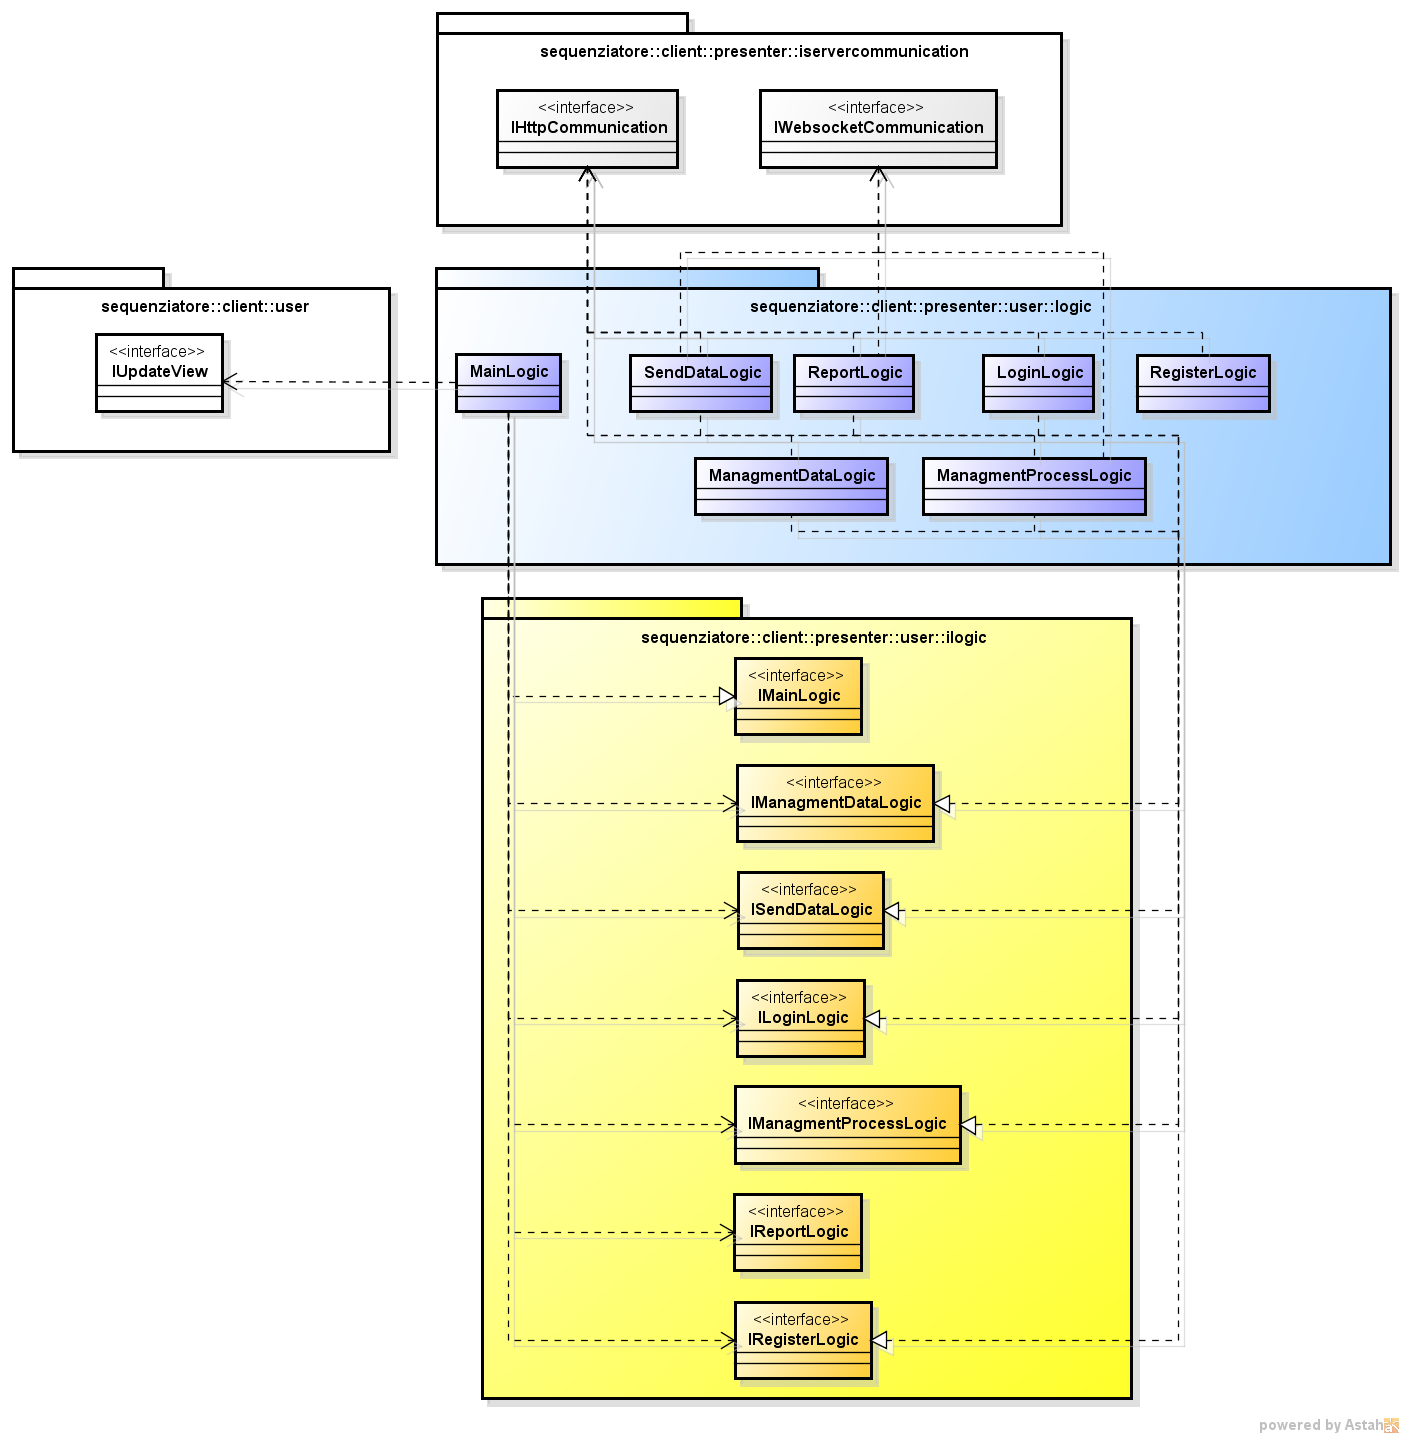
\includegraphics[width=%
\textwidth]
{./pack/presenter_user.png} \caption{Diagramma presenter user}
\end{figure}
\paragraph{IMainLogic}
\begin{itemize}
\item \textbf{Nome:} \texttt{IMainLogic};
\item \textbf{Package:} \texttt{\iLogicUser{}};
\item \textbf{Descrizione:} Interfaccia che permette di gestire gli eventi generati dalla componente \textit{View}.
\end{itemize}

\paragraph{ILoginLogic}
\begin{itemize}
\item \textbf{Nome:} \texttt{ILoginLogic};
\item \textbf{Package:} \texttt{\iLogicUser{}};
\item \textbf{Descrizione:} Interfaccia che ha il compito di gestire le richieste di autenticazione e chiusura della sessione da parte dell'utente.
\end{itemize}

\paragraph{IRegisterLogic}
\begin{itemize}
\item \textbf{Nome:} \texttt{IRegisterLogic};
\item \textbf{Package:} \texttt{\iLogicUser{}};
\item \textbf{Descrizione:} Interfaccia che ha il compito di gestire le richieste di registrazione da parte dell'utente.
\end{itemize}

\paragraph{IManagmentDataLogic}
\begin{itemize}
\item \textbf{Nome:} \texttt{IManagmentDataLogic};
\item \textbf{Package:} \texttt{\iLogicUser{}};
\item \textbf{Descrizione:} Interfaccia che ha il compito di gestire la visualizzazione e la modifica dei dati dell'utente.
\end{itemize}

\paragraph{IManagmentProcessLogic}
\begin{itemize}
\item \textbf{Nome:} \texttt{IManagmentProcessLogic};
\item \textbf{Package:} \texttt{\iLogicUser{}};
\item \textbf{Descrizione:} Interfaccia che ha il compito di gestire e accedere alle informazioni relative allo stato dei processi.
\end{itemize}

\paragraph{ISendDataLogic}
\begin{itemize}
\item \textbf{Nome:} \texttt{ISendDataLogic};
\item \textbf{Package:} \texttt{\iLogicUser{}};
\item \textbf{Descrizione:} Interfaccia che ha il compito di gestire l'inserimento e l'invio di dati da parte degli utenti.
\end{itemize}

\paragraph{IReportLogic}
\begin{itemize}
\item \textbf{Nome:} \texttt{IReportLogic};
\item \textbf{Package:} \texttt{\iLogicUser{}};
\item \textbf{Descrizione:} Interfaccia che ha il compito di gestire la creazione di report sull'andamento dei processi in esecuzione.
\end{itemize}
\subsubsection{Package sequenziatore::client::ipresenter::iprocessowner::ilogic}
\paragraph{IIMainLogic}
\begin{itemize}
\item \textbf{Nome:} \texttt{IMainLogic};
\item \textbf{Package:} \texttt{\iLogicAdmin{}};
\item \textbf{Descrizione:} Interfaccia che permette di gestire gli eventi generati dalla componente \textit{View};
\end{itemize}

\paragraph{ILoginLogic}
\begin{itemize}
\item \textbf{Nome:} \texttt{ILoginLogic};
\item \textbf{Package:} \texttt{\iLogicAdmin{}};
\item \textbf{Descrizione:} Interfaccia che ha il compito di gestire le richieste di autenticazione e chiusura della sessione da parte dell'utente \textit{process owner}.
\end{itemize}

\paragraph{INewProcessLogic}
\begin{itemize}
\item \textbf{Nome:} \texttt{INewProcessLogic};
\item \textbf{Package:} \texttt{\iLogicAdmin{}};
\item \textbf{Descrizione:} Interfaccia che ha il compito di gestire la logica della definizione di un nuovo processo.
\end{itemize}


\paragraph{IAddStepLogic}
\begin{itemize}
\item \textbf{Nome:} \texttt{IAddStepLogic};
\item \textbf{Package:} \texttt{\iLogicAdmin{}};
\item \textbf{Descrizione:} Interfaccia che ha il compito di definire la logica di gestione dei passi di un processo.
\end{itemize}


\paragraph{IManagmentProcessLogic}

\begin{itemize}
\item \textbf{Nome:} \texttt{IManagmentProcessLogic};
\item \textbf{Package:} \texttt{\iLogicAdmin{}};
\item \textbf{Descrizione:} Interfaccia che ha il compito di gestire e accedere alle informazioni relative allo stato dei processi.
\end{itemize}


\paragraph{ICheckStepLogic}
\begin{itemize}
\item \textbf{Nome:} \texttt{ICheckStepLogic};
\item \textbf{Package:} \texttt{\iLogicAdmin{}};
\item \textbf{Descrizione:} Interfaccia che ha il compito di definire la logica del controllo di un passo che richiede intervento umano per essere approvato.
\end{itemize}


\paragraph{IStatisticLogic}
\begin{itemize}
\item \textbf{Nome:} \texttt{IStatisticLogic};
\item \textbf{Package:} \texttt{\iLogicAdmin{}};
\item \textbf{Descrizione:} Interfaccia che ha il compito di gestire l'accesso alle informazioni statistiche sui processi.
\end{itemize}


\paragraph{IUserDataLogic}
\begin{itemize}
\item \textbf{Nome:} \texttt{IUserDataLogic};
\item \textbf{Package:} \texttt{\iLogicAdmin{}};
\item \textbf{Descrizione:} Interfaccia che ha il compito gestire l'accesso alle informazioni sui passi superati dagli utenti.
\end{itemize}


\paragraph{IInviteUserLogic}
\begin{itemize}
\item \textbf{Nome:} \texttt{IInviteUserLogic};
\item \textbf{Package:} \texttt{\iLogicAdmin{}};
\item \textbf{Descrizione:} Interfaccia che ha il compito di gestire i permessi di iscrizione ad un processo degli utenti.
\end{itemize}


\subsubsection{sequenziatore::client::ipresenter::iservercommunication}

\paragraph{IHttpCommunication}
\begin{itemize}
\item \textbf{Nome:} \texttt{IHttpCommunication};
\item \textbf{Package:} \texttt{\serverCommunication{}};
\item \textbf{Descrizione:} Interfaccia che permette di gestire l'invio e ricezione di dati al \textit{server\ped{G}} tramite protocollo HTTP\ped{G}.
\end{itemize}

\paragraph{IWebsocketCommunication}
\begin{itemize}
\item \textbf{Nome:} \texttt{IWebsocketCommunication};
\item \textbf{Package:} \texttt{\serverCommunication{}};
\item \textbf{Descrizione:} Interfaccia che permette di gestire l'invio e ricezione di dati dal \textit{server\ped{G}} tramite \textit{websocket\ped{G}}.
\end{itemize}

\paragraph{IDataFormatter}
\begin{itemize}
\item \textbf{Nome:} \texttt{IDataFormatter};
\item \textbf{Package:} \texttt{\serverCommunication{}};
\item \textbf{Descrizione:} Interfaccia che permette di gestire la formattazione dei dati da inviare e ricevuti dal \textit{server\ped{G}}.
\end{itemize}

\subsection{Package sequenziatore::client::presenter}
\subsubsection{Package sequenziatore::client::presenter::user::logic}

\paragraph{MainLogic}
\begin{flushleft}
\begin{itemize}
\item \textbf{Nome:} \texttt{MainLogic};
\item \textbf{Package:} \texttt{\logicUser{}};
\item \textbf{Descrizione:} Classe che permette di gestire gli eventi generati dalla componente \textit{View};
\item \textbf{Relazioni con altri componenti:}
\begin{sloppypar}
La classe implementa l'interfaccia \texttt{\iLogicUser{}::I\fshyp{}Main\fshyp{}Lo\fshyp{}gic} e delega la gestione della logica di dettaglio alle seguenti classi:
\end{sloppypar}
\begin{itemize}
\item \texttt{\logicUser{}::Lo\fshyp{}gin\fshyp{}Lo\fshyp{}gic};
\item \texttt{\logicUser{}::Re\fshyp{}gis\fshyp{}ter\fshyp{}Lo\fshyp{}gic};
\item \texttt{\logicUser{}::Ma\fshyp{}nag\fshyp{}ment\fshyp{}Da\fshyp{}ta\fshyp{}Lo\fshyp{}gic};
\item \texttt{\logicUser{}::Ma\fshyp{}nag\fshyp{}ment\fshyp{}Pro\fshyp{}cess\fshyp{}Lo\fshyp{}gic};
\item \texttt{\logicUser{}::Send\fshyp{}Da\fshyp{}ta\fshyp{}Lo\fshyp{}gic};
\item \texttt{\logicUser{}::Re\fshyp{}port\fshyp{}Lo\fshyp{}gic};
\end{itemize}
\end{itemize}
\end{flushleft}

\paragraph{LoginLogic}
\begin{flushleft}
\begin{itemize}
\item \textbf{Nome:} \texttt{LoginLogic};
\item \textbf{Package:} \texttt{\logicUser{}};
\item \textbf{Descrizione:} Classe che ha il compito di gestire le richieste di autenticazione e chiusura della sessione da parte dell'utente;
\item \textbf{Relazioni con altri componenti:}
\begin{sloppypar}
La classe implementa l'interfaccia \texttt{\iLogicUser{}::I\fshyp{}Log\fshyp{}in\fshyp{}Lo\fshyp{}gic}, e utilizza metodi delle classi \texttt{\serverCommunication{}::Http\fshyp{}Com\fshyp{}mu\fshyp{}ni\fshyp{}ca\fshyp{}tion} e \texttt{\viewUser{}::Up\fshyp{}da\fshyp{}te\fshyp{}View}.
\end{sloppypar}
\end{itemize}
\end{flushleft}

\paragraph{RegisterLogic}
\begin{flushleft}
\begin{itemize}
\item \textbf{Nome:} \texttt{RegisterLogic};
\item \textbf{Package:} \texttt{\logicUser{}};
\item \textbf{Descrizione:} Classe che ha il compito di gestire le richieste di registrazione da parte dell'utente;
\item \textbf{Relazioni con altri componenti:}
\begin{sloppypar}
La classe implementa l'interfaccia \texttt{\iLogicUser{}::I\fshyp{}Re\fshyp{}gis\fshyp{}ter\fshyp{}Lo\fshyp{}gic}, e utilizza metodi delle classi \texttt{\serverCommunication{}::Http\fshyp{}Com\fshyp{}mu\fshyp{}ni\fshyp{}ca\fshyp{}tion} e \texttt{\viewUser{}::Up\fshyp{}da\fshyp{}te\fshyp{}View}.
\end{sloppypar}
\end{itemize}
\end{flushleft}

\paragraph{ManagmentDataLogic}
\begin{flushleft}
\begin{itemize}
\item \textbf{Nome:} \texttt{ManagmentDataLogic};
\item \textbf{Package:} \texttt{\logicUser{}};
\item \textbf{Descrizione:} Classe che ha il compito di gestire la visualizzazione e la modifica dei dati dell'utente;
\item \textbf{Relazioni con altri componenti:}
\begin{sloppypar}
La classe implementa l'interfaccia \texttt{\iLogicUser{}::I\fshyp{}Ma\fshyp{}na\fshyp{}gment\fshyp{}Da\fshyp{}ta\fshyp{}Lo\fshyp{}gic}, e utilizza metodi delle classi \texttt{\serverCommunication{}::Http\fshyp{}Com\fshyp{}mu\fshyp{}ni\fshyp{}ca\fshyp{}tion} e \texttt{\viewUser{}::Up\fshyp{}da\fshyp{}te\fshyp{}View}.
\end{sloppypar}
\end{itemize}
\end{flushleft}

\paragraph{ManagmentProcessLogic}
\begin{flushleft}
\begin{itemize}
\item \textbf{Nome:} \texttt{ManagmentProcessLogic};
\item \textbf{Package:} \texttt{\logicUser{}};
\item \textbf{Descrizione:} Classe che ha il compito di gestire e accedere alle informazioni relative allo stato dei processi. Le operazioni di gestione dello stato comprendono l'eliminazione dei processi terminati;
\item \textbf{Relazioni con altri componenti:}
\begin{sloppypar}
La classe implementa l'interfaccia \texttt{\iLogicUser{}::I\fshyp{}Ma\fshyp{}na\fshyp{}gment\fshyp{}Pro\fshyp{}cess\fshyp{}Lo\fshyp{}gic}, e utilizza metodi delle classi 
\texttt{\serverCommunication{}::Http\fshyp{}Com\fshyp{}mu\fshyp{}ni\fshyp{}ca\fshyp{}tion}, 
\texttt{\serverCommunication{}::Web\fshyp{}so\fshyp{}cket\fshyp{}Com\fshyp{}mu\fshyp{}ni\fshyp{}ca\fshyp{}tion}, \texttt{\modelUser{}::U\fshyp{}ser\fshyp{}Da\fshyp{}ta} e 
\texttt{\viewUser{}::Up\fshyp{}da\fshyp{}te\fshyp{}View}.
\end{sloppypar}
\end{itemize}
\end{flushleft}

\paragraph{SendDataLogic}
\begin{flushleft}
\begin{itemize}
\item \textbf{Nome:} \texttt{SendDataLogic};
\item \textbf{Package:} \texttt{\logicUser{}};
\item \textbf{Descrizione:} Classe che ha il compito di gestire l'inserimento e l'invio di dati da parte degli utenti;
\item \textbf{Relazioni con altri componenti:}
\begin{sloppypar}
La classe implementa l'interfaccia \texttt{\iLogicUser{}::I\fshyp{}Send\fshyp{}Da\fshyp{}ta\fshyp{}Lo\fshyp{}gic}, e utilizza metodi delle classi \texttt{\serverCommunication{}::Http\fshyp{}Com\fshyp{}mu\fshyp{}ni\fshyp{}ca\fshyp{}tion}, \texttt{\serverCommunication{}::Web\fshyp{}so\fshyp{}cket\fshyp{}Com\fshyp{}mu\fshyp{}ni\fshyp{}ca\fshyp{}tion}, \texttt{\model{}::U\fshyp{}ser\fshyp{}Da\fshyp{}ta} e \texttt{\viewUser{}::Up\fshyp{}da\fshyp{}te\fshyp{}View}.
\end{sloppypar}
\end{itemize}
\end{flushleft}

\paragraph{ReportLogic}
\begin{flushleft}
\begin{itemize}
\item \textbf{Nome:} \texttt{ReportLogic};
\item \textbf{Package:} \texttt{\logicUser{}};
\item \textbf{Descrizione:} Classe che ha il compito di gestire la creazione di report sull'andamento dei processi in esecuzione;
\item \textbf{Relazioni con altri componenti:}
\begin{sloppypar}
La classe implementa l'interfaccia \texttt{\iLogicUser{}::I\fshyp{}Ma\fshyp{}na\fshyp{}gment\fshyp{}Lo\fshyp{}gic}, e utilizza metodi delle classi \texttt{\serverCommunication{}::HttpCommunication}, \texttt{\serverCommunication{}::Web\fshyp{}so\fshyp{}cket\fshyp{}Com\fshyp{}mu\fshyp{}ni\fshyp{}ca\fshyp{}tion}, \texttt{\modelUser{}::U\fshyp{}ser\fshyp{}Da\fshyp{}ta} \texttt{\viewUser{}::Up\fshyp{}da\fshyp{}te\fshyp{}View}.
\end{sloppypar}
\end{itemize}
\end{flushleft}
\subsubsection{sequenziatore::client::presenter::processowner::logic}
\paragraph{MainLogic}
\begin{flushleft}
\begin{itemize}
\item \textbf{Nome:} \texttt{MainLogic};
\item \textbf{Package:} \texttt{\logicAdmin{}};
\item \textbf{Descrizione:} Classe che permette di gestire gli eventi generati dalla componente \textit{View};
\item \textbf{Relazioni con altri componenti:}
\begin{sloppypar}
La classe implementa l'interfaccia \texttt{\iLogicAdmin{}.I\fshyp{}Main\fshyp{}Lo\fshyp{}gic} e delega la gestione della logica di dettaglio alle seguenti classi:
\end{sloppypar}
\begin{itemize}
\item \texttt{\logicAdmin{}::Lo\fshyp{}gin\fshyp{}Lo\fshyp{}gic};
\item \texttt{\logicAdmin{}::New\fshyp{}Pro\fshyp{}cess\fshyp{}Lo\fshyp{}gic};
\item \texttt{\logicAdmin{}::Add\fshyp{}Step\fshyp{}Lo\fshyp{}gic};
\item \texttt{\logicAdmin{}::Ma\fshyp{}nag\fshyp{}ment\fshyp{}Pro\fshyp{}cess\fshyp{}Lo\fshyp{}gic};
\item \texttt{\logicAdmin{}::Check\fshyp{}Step\fshyp{}Lo\fshyp{}gic};
\item \texttt{\logicAdmin{}::Sta\fshyp{}tis\fshyp{}tics\fshyp{}Lo\fshyp{}gic};
\item \texttt{\logicAdmin{}::U\fshyp{}ser\fshyp{}Da\fshyp{}ta\fshyp{}Lo\fshyp{}gic};
\item \texttt{\logicAdmin{}::In\fshyp{}vi\fshyp{}te\fshyp{}U\fshyp{}ser\fshyp{}Lo\fshyp{}gic}.
\end{itemize}
\end{itemize}
\end{flushleft}

\paragraph{UpdateView}
\begin{flushleft}
\begin{itemize}
\item \textbf{Nome:} \texttt{LoginLogic};
\item \textbf{Package:} \texttt{\logicAdmin{}};
\item \textbf{Descrizione:} Classe che ha il compito di gestire l'aggiornameno dei \textit{widget\ped{G}} della componente \textit{View};
\item \textbf{Relazioni con altri componenti:}
\begin{sloppypar}
La classe implementa l'interfaccia \texttt{\iLogicAdmin{}::I\fshyp{}Up\fshyp{}date\fshyp{}View} e comunica con la \textit{View} utilizzando metodi della classe \texttt{\viewAdmin{}::Up\fshyp{}da\fshyp{}te\fshyp{}View}.
\end{sloppypar}
\end{itemize}
\end{flushleft}

\paragraph{LoginLogic}
\begin{flushleft}
\begin{itemize}
\item \textbf{Nome:} \texttt{LoginLogic};
\item \textbf{Package:} \texttt{\logicAdmin{}};
\item \textbf{Descrizione:} Classe che ha il compito di gestire le richieste di autenticazione e chiusura della sessione da parte dell'utente \textit{process owner};
\item \textbf{Relazioni con altri componenti:}
\begin{sloppypar}
La classe implementa l'interfaccia \texttt{\iLogicAdmin{}::I\fshyp{}Log\fshyp{}in\fshyp{}Lo\fshyp{}gic}, e utilizza metodi delle classi \texttt{\serverCommunication{}::Http\fshyp{}Com\fshyp{}mu\fshyp{}ni\fshyp{}ca\fshyp{}tion} e \texttt{\logicAdmin{}::Up\fshyp{}da\fshyp{}te\fshyp{}View}.
\end{sloppypar}
\end{itemize}
\end{flushleft}

\paragraph{NewProcessLogic}
\begin{flushleft}
\begin{itemize}
\item \textbf{Nome:} \texttt{NewProcessLogic};
\item \textbf{Package:} \texttt{\logicAdmin{}};
\item \textbf{Descrizione:} Classe che ha il compito di gestire la logica della definizione di un nuovo processo, comunicando con il \textit{server\ped{G}} quando richiesto;
\item \textbf{Relazioni con altri componenti:}
\begin{sloppypar}
La classe implementa l'interfaccia \texttt{\iLogicAdmin{}::I\fshyp{}New\fshyp{}Pro\fshyp{}cess\fshyp{}Lo\fshyp{}gic}, e utilizza metodi delle classi \texttt{\serverCommunication{}::Http\fshyp{}Com\fshyp{}mu\fshyp{}ni\fshyp{}ca\fshyp{}tion}, \texttt{\serverCommunication{}::Web\fshyp{}so\fshyp{}cket\fshyp{}Com\fshyp{}mu\fshyp{}ni\fshyp{}ca\fshyp{}tion}, \texttt{\modelAdmin{}::Pro\fshyp{}cess} e \texttt{\logicAdmin{}::Up\fshyp{}da\fshyp{}te\fshyp{}View}.
\end{sloppypar}
\end{itemize}
\end{flushleft}

\paragraph{AddStepLogic}
\begin{flushleft}
\begin{itemize}
\item \textbf{Nome:} \texttt{AddStepLogic};
\item \textbf{Package:} \texttt{\logicAdmin{}};
\item \textbf{Descrizione:} Classe che ha il compito di definire la logica di gestione dei passi di un processo;
\item \textbf{Relazioni con altri componenti:}
\begin{sloppypar}
La classe implementa l'interfaccia \texttt{\iLogicAdmin{}::I\fshyp{}Add\fshyp{}Step\fshyp{}Lo\fshyp{}gic}, e utilizza metodi delle classi \texttt{\model{}::Step} e \texttt{\logicAdmin{}::Up\fshyp{}da\fshyp{}te\fshyp{}View}.
\end{sloppypar}
\end{itemize}
\end{flushleft}

\paragraph{ManagmentProcessLogic}
\begin{flushleft}
\begin{itemize}
\item \textbf{Nome:} \texttt{ManagmentProcessLogic};
\item \textbf{Package:} \texttt{\logicAdmin{}};
\item \textbf{Descrizione:} Classe che ha il compito di gestire e accedere alle informazioni relative allo stato dei processi. Le operazioni di gestione dello stato comprendono la terminazione e l'eliminazione di un processo;
\item \textbf{Relazioni con altri componenti:}
\begin{sloppypar}
La classe implementa l'interfaccia \texttt{\iLogicAdmin{}::I\fshyp{}Ma\fshyp{}na\fshyp{}gment\fshyp{}Lo\fshyp{}gic}, e utilizza metodi delle classi \texttt{\serverCommunication{}::HttpCommunication}, \texttt{\serverCommunication{}::WebsocketCommunication}, \texttt{\modelAdmin{}::Pro\fshyp{}cess} e \texttt{\logicAdmin{}::Up\fshyp{}da\fshyp{}te\fshyp{}View}.
\end{sloppypar}
\end{itemize}
\end{flushleft}

\paragraph{CheckStepLogic}
\begin{flushleft}
\begin{itemize}
\item \textbf{Nome:} \texttt{CheckStepLogic};
\item \textbf{Package:} \texttt{\logicAdmin{}};
\item \textbf{Descrizione:} Classe che ha il compito di definire la logica del controllo di un passo che richiede intervento umano per essere approvato;
\item \textbf{Relazioni con altri componenti:}
\begin{sloppypar}
La classe implementa l'interfaccia \texttt{\iLogicAdmin{}::I\fshyp{}Check\fshyp{}Step\fshyp{}Lo\fshyp{}gic}, e utilizza metodi delle classi \texttt{\serverCommunication{}::Http\fshyp{}Com\fshyp{}mu\fshyp{}ni\fshyp{}ca\fshyp{}tion}, \texttt{\serverCommunication{}::Web\fshyp{}so\fshyp{}cket\fshyp{}Com\fshyp{}mu\fshyp{}ni\fshyp{}ca\fshyp{}tion}, \texttt{\modelAdmin{}::Step} e \texttt{\logicAdmin{}::Up\fshyp{}da\fshyp{}te\fshyp{}View}.
\end{sloppypar}
\end{itemize}
\end{flushleft}

\paragraph{StatisticLogic}
\begin{flushleft}
\begin{itemize}
\item \textbf{Nome:} \texttt{StatisticLogic};
\item \textbf{Package:} \texttt{\logicAdmin{}};
\item \textbf{Descrizione:} Classe che ha il compito di gestire l'accesso alle informazioni statistiche sui processi, come il numero di utenti partecipanti e il numero di completamenti;
\item \textbf{Relazioni con altri componenti:}
\begin{sloppypar}
La classe implementa l'interfaccia \texttt{\iLogicAdmin{}::I\fshyp{}Sta\fshyp{}tis\fshyp{}tic\fshyp{}Lo\fshyp{}gic}, e utilizza metodi delle classi \texttt{\serverCommunication{}::Http\fshyp{}Com\fshyp{}mu\fshyp{}ni\fshyp{}ca\fshyp{}tion}, \texttt{\modelAdmin{}::Pro\fshyp{}cess}, \texttt{\model{}::Step} e \texttt{\logicAdmin{}::Up\fshyp{}da\fshyp{}te\fshyp{}View}.
\end{sloppypar}
\end{itemize}
\end{flushleft}

\paragraph{UserDataLogic}
\begin{flushleft}
\begin{itemize}
\item \textbf{Nome:} \texttt{UserDataLogic};
\item \textbf{Package:} \texttt{\logicAdmin{}};
\item \textbf{Descrizione:} Classe che ha il compito gestire l'accesso alle informazioni sui passi superati dagli utenti;
\item \textbf{Relazioni con altri componenti:}
\begin{sloppypar}
La classe implementa l'interfaccia \texttt{\iLogicAdmin{}::I\fshyp{}U\fshyp{}ser\fshyp{}Da\fshyp{}ta\fshyp{}Lo\fshyp{}gic}, e utilizza metodi delle classi \texttt{\serverCommunication{}::Http\fshyp{}Com\fshyp{}mu\fshyp{}ni\fshyp{}ca\fshyp{}tion}, \texttt{\modelAdmin{}::Pro\fshyp{}cess}, \texttt{\model{}::Step} e \texttt{\logicAdmin{}::Up\fshyp{}da\fshyp{}te\fshyp{}View}.
\end{sloppypar}
\end{itemize}
\end{flushleft}

\paragraph{InviteUserLogic}
\begin{flushleft}
\begin{itemize}
\item \textbf{Nome:} \texttt{InviteUserLogic};
\item \textbf{Package:} \texttt{\logicAdmin{}};
\item \textbf{Descrizione:} Classe che ha il compito di gestire i permessi di iscrizione ad un processo degli utenti;
\item \textbf{Relazioni con altri componenti:}
\begin{sloppypar}
La classe implementa l'interfaccia \texttt{\iLogicAdmin{}::I\fshyp{}In\fshyp{}vi\fshyp{}te\fshyp{}U\fshyp{}ser\fshyp{}Lo\fshyp{}gic}, e utilizza metodi delle classi \texttt{\serverCommunication{}::Http\fshyp{}Com\fshyp{}mu\fshyp{}ni\fshyp{}ca\fshyp{}tion}, \texttt{\serverCommunication{}::Web\fshyp{}so\fshyp{}cket\fshyp{}Com\fshyp{}mu\fshyp{}ni\fshyp{}ca\fshyp{}tion} e \texttt{\logicAdmin{}::Up\fshyp{}da\fshyp{}te\fshyp{}View}.
\end{sloppypar}
\end{itemize}
\end{flushleft}

\subsubsection{sequenziatore::client::presenter::servercommunication}

\paragraph{HttpCommunication}
\begin{flushleft}
\begin{itemize}
\item \textbf{Nome:} \texttt{HttpCommunication};
\item \textbf{Package:} \texttt{\serverCommunication{}};
\item \textbf{Descrizione:} Classe che permette di gestire l'invio e ricezione di dati al \textit{server\ped{G}} tramite protocollo HTTP\ped{G};
\item \textbf{Relazioni con altri componenti:}
\begin{sloppypar}
La classe implementa l'interfaccia \texttt{\iServerCommunication{}::I\fshyp{}Http\fshyp{}Com\fshyp{}mu\fshyp{}ni\fshyp{}ca\fshyp{}tion} e formatta i dati da inviare e ricevuti tramite la classe \texttt{\serverCommunication{}::JSON\fshyp{}For\fshyp{}mat\fshyp{}ter}.
\end{sloppypar}
\end{itemize}
\end{flushleft}

\paragraph{WebsocketCommunication}
\begin{flushleft}
\begin{itemize}
\item \textbf{Nome:} \texttt{WebsocketCommunication};
\item \textbf{Package:} \texttt{\serverCommunication{}};
\item \textbf{Descrizione:} Classe che permette di gestire l'invio e ricezione di dati dal \textit{server\ped{G}} tramite \textit{websocket\ped{G}};
\item \textbf{Relazioni con altri componenti:}
\begin{sloppypar}
La classe implementa l'interfaccia \texttt{\iServerCommunication{}::I\fshyp{}Web\fshyp{}so\fshyp{}cket\fshyp{}Com\fshyp{}mu\fshyp{}ni\fshyp{}ca\fshyp{}tion} e formatta i dati da inviare e ricevuti tramite la classe \texttt{\serverCommunication{}::JSON\fshyp{}For\fshyp{}mat\fshyp{}ter}.
\end{sloppypar}
\end{itemize}
\end{flushleft}

\paragraph{JSONFormatter}
\begin{flushleft}
\begin{itemize}
\item \textbf{Nome:} \texttt{JSONFormatter};
\item \textbf{Package:} \texttt{\serverCommunication{}};
\item \textbf{Descrizione:} Classe che permette di gestire la formattazione dei dati da inviare e ricevuti dal \textit{server\ped{G}};
\item \textbf{Relazioni con altri componenti:}
\begin{sloppypar}
La classe implementa l'interfaccia \texttt{\iServerCommunication{}::I\fshyp{}Da\fshyp{}ta\fshyp{}For\fshyp{}mat\fshyp{}ter}.
\end{sloppypar}
\end{itemize}
\end{flushleft}
